
\documentclass[twocolumn]{aastex63}
%% \documentclass[arguments]{aastex63}
%%
%% \documentclass[twocolumn,linenumbers,trackchanges]{aastex63}
%%
\newcommand\aastex{AAS\TeX}
\newcommand\latex{La\TeX}
%\include{subcaption}
%\usepackage{caption}

\shorttitle{Galaxian Contamination in Galactic Reddening Maps}
\shortauthors{Brown \& Walker}
%%

\begin{document}

\title{Galaxian Contamination in Galactic Reddening Maps}


\correspondingauthor{Peter J. Brown}
\email{pbrown@physics.tamu.edu}

\author[0000-0001-6272-5507]{Peter J. Brown}
\affil{Department of Physics and Astronomy,
Texas A\&M University, 4242 TAMU, College Station, TX 77843, USA }
\affil{George P. and Cynthia Woods Mitchell Institute for Fundamental Physics \& Astronomy}

\author{Tate Walker}
\affil{Department of Aerospace Engineering,
Texas A\&M University, 4242 TAMU, College Station, TX 77843, USA }


\begin{abstract}

Estimating the amount of foreground extinction due to the Milky Way dust along the line of sight is often a first step in determining the luminosity of an object.  The amount of Galactic dust inferred by infrared emission maps can be contaminated by infrared light from nearby galaxies.  By comparing extinction values at and around the location of nearby galaxies, we compile a list of 95 galaxies which likely contaminate the maps with an excess or improperly-subtracted galaxian infrared emission and tabulate our recommend values for the MW contribution.  In addition to M82, which inspired this work, six more sources have an excess visual extinction A$_V$ of at least 0.05 mag greater than our annular values, including M83, NGC1313, NGC6822, NGC918, UGC11501, and  UGC11797. M33 is shown to be oversubtracted. NGC88 and the outskirts of NGC4258 are located in gaps in the IRAS imaging.  The recommended dust map values for the LMC, SMC, and M31 may also not be correctly returned by some software packages. Accurate reddening estimates are important for measuring stellar and supernova luminosities in these nearby galaxies.

\end{abstract}

\keywords{dust: general, Milky Way: dust}


\section{Introduction} \label{sec:intro}

As luminosity is a fundamental property of astrophysical objects, properly correcting for the extinction of light due to dust is important.  Accurate luminosities are needed for calculating energy budgets, sizes of objects, and the calibration and use of astrophysical objects as standard candles to measure distances in the universe.

Dust extinction can occur anywhere along the line of sight from an object to the observer, including circumstellar dust, dust in the host galaxy of an object, circumgalactic dust, intergalactic dust, and dust in our own Milky Way galaxy.  These multiple components can make a full determination of the extinction complicated, but it is usually assumed that the component of dust extinction arising from the MW is the best understood.  The all-sky dust reddening maps of \citet{Schlegel_etal_1998}, hereafter referred to as SFD98, improved on the earlier HI estimates of \citet{Burstein_Heiles_1982} by  calibrating the luminosity at 100 $\mu$m from the Diffuse InfraRed Background Experiment on the Cosmic Background Explorer (DIRBE/COBE) and the Infrared Astronomical Satellite (IRAS) and converting it into the V-band extinction using the colors of elliptical galaxies.  These maps have made it convenient to look up the SFD98 reddening (or the rescaling by
\citealp{Schlafly_Finkbeiner_2011}) via the NASA Extragalactic Database (NED\footnote{\url{https://ned.ipac.caltech.edu/}}; \citealp{Mazzarella_etal_2001}) 
or other electronic queries without having to understand the data,  read the paper, or notice the warnings from NED\footnote{\url{https://ned.ipac.caltech.edu/classic/help/faq3.html\#3a}}.  Combined with the mean value of R$_V$=3.1 from \citet{Fitzpatrick_1999}, one can compute the extinction as a function of wavelength or at the effective wavelength of a filter for a particular source.
%and ignoring the variations in the Milky Way \citep{Clayton_Cardelli_1988} one has the extinction as a function of wavelength or can also implicitly assume those as well as the elliptical galaxy spectrum used by SFD98 and have the extinction readily computed in a number of common passbands.  
Such ease, however, often makes it too easy to overlook the details and complications extant in the data set.

 \citet{Dalcanton_etal_2009} mentioned in a footnote that the SFD98 maps were clearly contaminated by M82, brought to our knowledge through studies of the extinction toward the supernova (SN) 2014J \citep{Foley_etal_2014J}.  \citet{Johnson_etal_2009} cautioned about not just the contamination of M81 and M82 but also the highly variable region nearby.  \citet{Chiang_Menard_2019} found that even distant galaxy clusters leave a small imprint on the dust maps. As dust reddening from anywhere has strong consequences in the ultraviolet, the authors were led to ask the question ``Which nearby galaxies might be contaminating the dust maps in this same way?''

In this short paper we describe how we searched for examples of contaminating galaxies and give a table of recommended extinction values for the ones we found.  


%%%%%%%%%%%%%%%%%%%%%%%%%%%%%%%%%%%%%%%%%%
\section{Analysis} \label{sec_analysis}
  

%Having one example to work from, the nearby, extreme starburst galaxy M82, we began our search by looking at the next eleven closest galaxies hosting supernovae observed by Swift (see e.g. \citealp{Brown_etal_2015_10}).  

To detect likely point sources from galaxy contaminants in the dust maps, we searched for excesses in A$_V$ at the center of each galaxy of interest compared to the mean of the values 20\arcmin\ away in each of the four cardinal directions.  We could then individually examine sources which were significantly higher than the mean of the 20\arcmin\ radius.  As a baseline for what a significant excess is, we first looked up the A$_V$ values (via IrsaDust.get\_extinction\_table in the Astroquery Python package) for 102 random positions in the sky.  The central and mean radial values are plotted in Figure \ref{fig_av}.  
As expected, most of the points cluster around the 1:1 line compared to the mean value in the surrounding points, and the scatter is a consistent fraction of the central value (note that both axis are on a log scale).  From the random positions, we set one and two sigma limits of 12\% and 22\% which encompass 68\% and 95\% of the points, respectively. 
A few points lie significantly below the 1:1 line due to bright spots in the angular regions.  


\begin{figure}
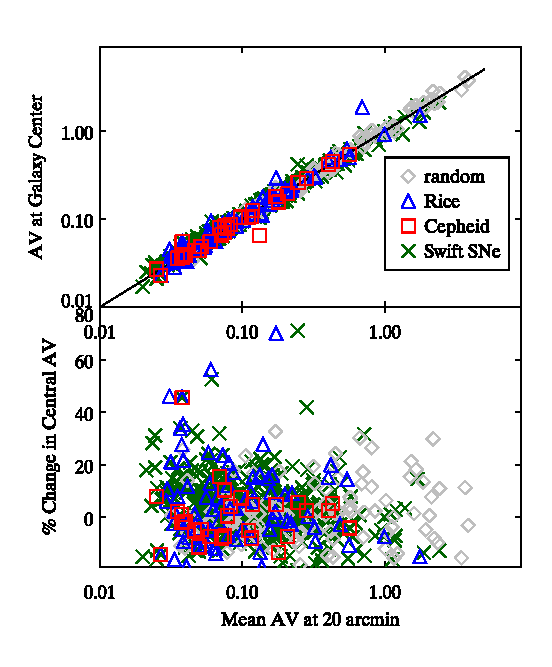
\includegraphics{avboth.eps}
\caption{Top panel: The central value of A$_V$ is plotted with respect to the mean of the A$_V$ values 20\arcmin\ away in each of the four cardinal directions.  102 random positions are plotted in grey.  The sample from \citet{Rice_etal_1988} which should have already been removed are blue triangles.  Nearby galaxies used to calibrate the Cepheid-SN distance ladder \citep{Riess_etal_2016} are plotted as red squares.  The sample of Swift supernovae are green crosses.  A 1:1 line shows perfect agreement between the values.
Bottom panel: A$_V$ differences normalized by the mean A$_V$ at 20\arcmin.  The fractional difference is fairly constant with A$_V$.  
The fractional differences for the random locations have a standard deviation of 12\%.  This is used as the cutoff for our manual examination.
\label{fig_av}}
\end{figure}




We queried the A$_V$ values at the location of each of the extragalactic sources in \citet{Rice_etal_1988}, the 70 brightest of which should already have been removed from the SFD98 maps.  For our scientific purposes, we also tabulated the nearby host galaxies used to calibrate the Cepheid-Supernova Ia distance ladder \citep{Riess_etal_2016}, the SINGS sample \citep{Kennicutt_etal_2003}, and over 700 supernova host galaxies observed by Swift \citep{Brown_etal_2014_SOUSA}.   We manually examine the fields of all galaxies for which the central position has an A$_V$ of 12\% greater than the mean of the points at 20\arcmin~and all of the sources from \citet{Rice_etal_1988}.


For each galaxy above our excess threshold, a square InfraRed Space ATLAS image (based on IRAS imaging) 100 \micron\ image  80\arcmin\ across was created as well as a plot with the A$_V$ as a function of radius out to 20\arcmin\ in each of the cardinal directions in steps of 1\arcmin.  Examples are shown in Figure \ref{fig_images}.
Both of these were visually examined to assess if the central excess was likely due to the flux of the galaxy, part of a region with highly variable infrared flux from the MW, or both.  
%If the galaxy seemed to contribute to the excess, a value was chosen representing our best estimate of the $A_V$ at the galaxy location and a radius within which that value should be used.  For an isolated source, the $A_V$ corresponds to the background level.  For galaxies in a region with a highly-variable foreground MW IR emission, such as a gradient, patchy emission, or artifacts, this was more subjective and used the IRAS image as a guide.
If the galaxy seemed to contribute to the excess, a radius was determined at which the galaxian contribution dropped below the background level.  We then queried the $A_V$ values at 360 locations at that radius.  We report the median value and standard deviation of those values in Table 1.   For galaxies in a region with a highly-variable foreground MW IR emission, such as a gradient, patchy emission, or artifacts, more sophisticated two-dimensional modeling or cross correlation with other forms of reddening estimates might better sample the contaminated region. 
Though imperfect, we believe our values to more accurately reflect the true MW reddening at the location of the galaxies than the look up tables used based on \citet{Schlegel_etal_1998}.  

Some sources appear to be partially removed, replacing the pixels with the median value of a nearby annulus.  The replaced region, however, is in some cases too small and the replacement value too bright in the regions passing our cuts.  M51 and M83, as shown in Figure \ref{fig_images}, are two examples of this.
Visual examination of the \citet{Rice_etal_1988} galaxies was done to find galaxies with poor subtraction which nevertheless did not meet our criteria of having a significant central excess.  M33 is a striking example which appears to be oversubtracted, as shown in \ref{fig_images2}.  In many cases our recommended value is only slightly smaller than the map value ($\sim$0.01 mag), but its use may avoid a small bias.  In some instances, such as NGC2442 and NGC4666, our recommended value is close to the replacement value used in the maps.  The complexity of the location, however, leads to a higher recommended uncertainty, because the galaxy line of sight may or may not pass through the brighter regions of the foreground emission.  Including a higher uncertainty for these objects recognizes that our knowledge of the MW dust is not as complete as is often assumed.

Other values returned from the tools are not properly corrected for the suggested corrections for the nearby Large and Small Magellanic clouds and M31 given in Appendix C of SFD98.  
The recommended value for the region around M31, for example, is E(B-V)=0.062 (SFD98; 0.055 in the \citealp{Schlafly_Finkbeiner_2011} system).  The \citet{Schlafly_Finkbeiner_2011} value of 0.055 is obtained from the NASA Extragalactic Database\footnote{https://ned.ipac.caltech.edu/} when searching the position of M31.  Since M31 is not removed from the maps, however, one obtains a value of E(B-V)=0.60 (a factor of 10 larger) from the NASA/IPAC Infrared Science Archive from the website\footnote{https://irsa.ipac.caltech.edu/frontpage/} or Astroquery in python.  This field is shown in the second panel of Figure \ref{fig_images2}.


Another problematic field we found was in the region of NGC4258.  NGC4258 is an important rung of the extragalactic distance scale because of its geometrically-determined distance which is used either as a calibration of or a check of Cepheid distances \citep{Macri_etal_2006, Humphreys_etal_2013,Hoffmann_etal_2016, Reid_etal_2019}.
%\footnote{\citet{Fausnaugh_etal_2015} found an unusually grey extinction law for the Cepheids in NGC4258. It is beyond the scope of this paper to evaluate whether an incorrect value of the line of sight MW extinction could have a significant effect.}.  
There is a clear point source visible in some of the IRAS images.  In most of the images available from the NASA/Infrared Processing and Analysis Center (IPAC), however, NGC4258 falls in a gap between data.  This results in a discontinuity in the combined images.  The central value of A$_V$ derived from the maps is small and appears correct, so analyses using the galaxy value appear fine (e.g. \citealp{Macri_etal_2006}).  Using values at the positions of individual objects in the outer fields in the south and east could overestimate the small MW reddening by $\sim50\%$, as shown in  Figure \ref{fig_images2}.  This would be a small effect but potentially significant for objects with low host reddening in a science field where precision and accuracy are critical.  NGC88 also falls in a gap.  For both of these objects we provide a recommended value within a radius around the galaxy center based on values outside the gap.

 Reading the mask values from the SFD data product would catch some of the sources in or near the SMC, LMC, or M31 or for which no IRAS data existed and the COBE/DIRBE maps were used instead. 
These oversights could just be treated as a bug and corrected in these archives.  Since past work may have been incorrectly analyzed, we are publishing this research article as well as notifying the developers in order to promote the best science in past and future analyses.  

The list of contaminating galaxies is given in Table 1 with their central coordinates, the radius of contamination, our estimate for A$_V$, and our estimated uncertainty on A$_V$. 
The values for the LMC, SMC and M31 recommended by Appendix C of SFD98 are corrected to the \citet{Schlafly_Finkbeiner_2011} system and listed in Table 1 along with the recommended value for M82 from \citet{Dalcanton_etal_2009}.  Thus one could query this table by position in order to update MW reddening values obtained from the IR maps.  We note, however, that work requiring precise line of sight extinctions through these large areas should utilize other methods to better constrain the minimum position-dependent line of sight extinction contributed by the Milky Way in these extended areas (e.g. \citealp{Haschke_etal_2011}).



In this paper we have focused on the commonly-used SFD98 maps.  Visual inspection of the galaxies flagged in this analysis using the \citet{Planck_etal_2014} maps reveal the same issues of contamination.  The \citet{Planck_etal_2014} contamination is actually more severe because the extragalactic sources not in the point source catalog were not removed from the IRIS map, while most of the corrections discussed previously were for sources not fully subtracted in SFD98.  Our spot checks of significant sources found in SFD are also found in the \citet{Planck_etal_2014} dustmaps obtained through the dustmaps utility. We recommend that members of the Planck team who understand the data best make a best effort attempt to remove these extragalactic contaminants, possibly using two-dimensional interpolation, power spectra, or gaussian processes to better fill in the contaminated regions than the median-filled circles used here and by SFD.   Other methods of reddening determinations, such as stellar colors \citep{Green_etal_2019} and HI maps \citep{Lenz_etal_2017}, should also be consulted if a precise extinction is needed.  Understanding the limitations (such as low HI column density for HI reddening; \citealp{Lenz_etal_2017}) of any method is still important. 


Many corrections for extinction already utilize the intrinsic colors of an object (e.g. type Ia supernovae; \citealp{Phillips_etal_1999}) to determine the total reddening to it.  An incorrect measure of the MW reddening could be compensated by a larger or smaller value of the host galaxy reddening, yielding the same total extinction if the MW and host galaxy reddening laws are the same.  In the  limiting case of negligible host reddening the flux could be overcorrected, resulting in bluer colors which might be interpreted as zero or negative reddening depending on the assumed priors in the SN fitting.


\begin{figure*}
\begin{tabular}{cc}
 \includegraphics[width=65mm]{NGC918.png} &   \includegraphics[width=65mm]{NGC918e.png} \\
%(a) first & (b) second \\[6pt]
  \includegraphics[width=65mm]{NGC1371.png} &   \includegraphics[width=65mm]{NGC1371e.png} \\
%(c) third & (d) fourth \\[6pt]
 \includegraphics[width=65mm]{M51.png} &   \includegraphics[width=65mm]{M51e.png} \\
%(c) third & (d) fourth \\[6pt]
 \includegraphics[width=65mm]{M83.png} &   \includegraphics[width=65mm]{M83e.png} \\
%(c) third & (d) fourth \\[6pt]
\end{tabular}
\caption{100 \micron IRAS images (80\arcmin $\times$ 80\arcmin with North pointing up) on the left and the corresponding plots of A$_V$ v. distance from center for a few galaxies illustrating the range of contamination.  The top panel shows the small but clear contribution of NGC1371.  The second panel shows the more complicated field of NGC1448.  The bottom two panels show the uncomplete subtraction of M51 and M83.}\label{fig_images}
\end{figure*}



\begin{figure*}
\begin{tabular}{cc}
  \includegraphics[width=65mm]{M33.png} &   \includegraphics[width=65mm]{M33e.png} \\
%(a) first & (b) second \\[6pt]
 \includegraphics[width=65mm]{M31.png} &   \includegraphics[width=65mm]{M31e.png} \\
%(c) third & (d) fourth \\[6pt]
 \includegraphics[width=65mm]{NGC4258.png} &   \includegraphics[width=65mm]{NGC4258e.png} \\
%(c) third & (d) fourth \\[6pt]
 \includegraphics[width=65mm]{NGC88.png} &   \includegraphics[width=65mm]{NGC88e.png} \\
%(c) third & (d) fourth \\[6pt]
\end{tabular}
\caption{100 \micron IRAS images (80\arcmin $\times$ 80\arcmin with North pointing up) on the left and the corresponding plots of A$_V$ versus distance from center for a few galaxies illustrating the range of contamination. In the first row, M33 has been oversubtracted, so the MW reddening would be underestimated.  In the second panel, M31 has not been removed, with the recommended value from the appendix of SFD98 being reported by NED but not IRSA.  The bottom panels show discontinuities in the reddening values near NGC4258 and NGC88 due to data gaps in the IRAS imaging.  }\label{fig_images2}
\end{figure*}



%%%%%%%%%%%%%%%%%%%%%%%
\section{Summary\label{sec_summary}}

In summary, we have searched for galaxies whose infrared emission might significantly contaminate the IRAS images resulting in a overestimate of the foreground MW dust reddening.  We provide a table of such galaxies, their coordinates, our recommended values on the \citet{Schlafly_Finkbeiner_2011} system, and the radius with which to use replacement values from those looked up by default from the SFD98 maps via NED or Astroquery \citep{Ginsburg_etal_2019}.  This will be communicated to the developers of such tools, and we make available our code to query our table or the dust maps as appropriate\footnote{https://github.com/pbrown801/AV  https://doi.org/10.5281/zenodo.5547785}.  We recommend, however, that users make themselves aware of the issues of the data they use by reading the original papers even when the data products are made easily accessible via automated sources.

\acknowledgments
We appreciate useful discussions with D. Schlegel and D. Finkbeiner about the SFD98 maps and comments on the manuscript from N. Suntzeff.  Most of this work was done as a student project as part of Texas A\&M's Aggie Research Program.  This work was also supported by the Mitchell Institute for Fundamental Physics and Astronomy and NASA grant 80NSSC20K0456. 

% Facilities 

\vspace{5cm}
\facilities{(IRAS)}

\software{ astropy \citep{Astropy_2013,Astropy_2018}, astroquery \citep{Ginsburg_etal_2019}, scipy \citep{Scipy_2001,Scipy_2019} }

\clearpage

\bibliographystyle{aasjournal}
\bibliography{bibtex}{}

\clearpage
\begin{longrotatetable}
%% The values (usually only l,r and c) in the last part of
%% \begin{deluxetable}{} command tell LaTeX how many columns
%% there are and how to align them.
\begin{deluxetable*}{llrrrrrr}

%% Keep a portrait orientation

%% Over-ride the default font size
%% Use Default (12pt)

%% Use \tablewidth{?pt} to over-ride the default table width.
%% If you are unhappy with the default look at the end of the
%% *.log file to see what the default was set at before adjusting
%% this value.

%% This is the title of the table.
\tablecaption{Improved Estimates for the Galactic Extinction in the Line of Sight near External Galaxies in the  \citet{Schlafly_Finkbeiner_2011} System}

%% This command over-rides LaTeX's natural table count
%% and replaces it with this number.  LaTeX will increment 
%% all other tables after this table based on this number
\tablenum{1}

%% The \tablehead gives provides the column headers.  It
%% is currently set up so that the column labels are on the
%% top line and the units surrounded by ()s are in the 
%% bottom line.  You may add more header information by writing
%% another line between these lines. For each column that requries
%% extra information be sure to include a \colhead{text} command
%% and remember to end any extra lines with \\ and include the 
%% correct number of &s.
\tablehead{\colhead{Galaxy Name} & \colhead{RA} & \colhead{Dec} & \colhead{Radius} & \colhead{A$_V$} & \colhead{Err} & \colhead{Supernovae} \\ 
\colhead{} & \colhead{(H M S)} & \colhead{(D M S)} & \colhead{(arcsec)} & \colhead{(mag)} & \colhead{(mag)} & \colhead{(mag)} & \colhead{} } 
%%  4. The LMC, SMC, and M31 are not removed from the maps, nor are sources within their Holmberg radius. Accurate reddenings through these galaxies are not possible, since their temperature structure is not sufficiently resolved by DIRBE. Typical reddenings toward these galaxies are estimated from the median dust emission in surrounding annuli: E(B-V) = 0.075 mag for the LMC, 0.037 mag for the SMC, and 0.062 mag for M31.
%% All data must appear between the \startdata and \enddata commands
\startdata
LMC & 05h23m34.6s & -69d45m22s & 323 & 2.419 & 0.20\tablenotekey{(a)} & 0.05 & \nodata \\
SMC & 00h52m38.0s & -72d48m01s & 190 & 1.188 & 0.10\tablenotekey{(a)} & 0.05 & \nodata \\
M31 & 00h42m44.5s & +41d16m09s & 95 & 1.862 & 0.17\tablenotekey{(a)} & 0.05 & \nodata \\
M82 & 9h55m52.43s & 69d40m46.93s & 20 & 0.419 & 0.16\tablenotekey{(b)} & 0.05 & \nodata \\
Arp244 & 12h01m53.17s & -18d52m37.92s & 15 & 0.124 & 0.11 & 0.01 & SNe 1921A, 1974E, 2004gt, 2007sr, 2013dk \\
ESO138-G10 & 16h59m02.952s & -60d12m57.67s & 12 & 0.591 & 0.55 & 0.05 & SN2013by \\
ESO287-G40 & 21h37m28.1842s & -47d02m08.8331s & 7 & 0.077 & 0.065 & 0.01 & SNe 2009lc, 2013fy\\
ESO317-32 & 10h28m01.6186s & -42d06m38.7541s & 12 & 0.363 & 0.33 & 0.03 & SN2017ghs\\
ESO509-IG064 & 13h34m39.3s & -23d40m50s & 15 & 0.339 & 0.3 & 0.02 & SN2016eiy\\
IC208 & 2h08m27.736s & 6d23m41.53s & 12 & 0.147 & 0.13 & 0.01 & SNe 2003G, 2017glq \\
IC2574 & 10h28m23.6205s & 68d24m43.4414s & 15 & 0.097 & 0.08 & 0.01 & \nodata \\
IC5249 & 22h47m06.262s & -64d49m55.42s & 15 & 0.092 & 0.08 & 0.01 & SN2011cb \\
KUG0647+311 & 6h50m36.832s & 31d07m00.6s & 15 & 0.356 & 0.31 & 0.03 & SN2016asf \\
M51 & 13h29m52.698s & 47d11m42.93s & 15 & 0.094 & 0.05 & 0.01 & SNe 1945A, 1994I, 2005cs, 2011dh\\
M61 & 12h21m54.9275s & 4d28m25.5883s & 15 & 0.06 & 0.05 & 0.01 & SNe 1926A, 1964F, 1961I, 1999gn, 2006ov, 2008in, 2014dt\\
M66 & 11h20m15.026s & 12d59m28.64s & 15 & 0.09 & 0.07 & 0.01 & SNe 1973R, 1989B, 1997bs, 2009hd, 2016cok \\
M74 & 1h36m41.772s & 15d47m00.46s & 15 & 0.188 & 0.16 & 0.02 & SNe 2002ap, 2003gd, 2013ej, PS15blm \\
M82 & 9h55m52.43s & 69d40m46.93s & 20 & 0.419 & 0.2 & 0.05 & SNe 2004am, 2008iz, 2014J, 2019aji\\
M83 & 13h37m00.919s & -29d51m56.74s & 15 & 0.178 & 0.12 & 0.01 & SNe 1923A, 1945B, 1950B, 1957D, 1968L, 1983N \\
MCG-01-07-004 & 2h23m13.2516s & -4d31m01.5168s & 7 & 0.08 & 0.07 & 0.05 & SNe ASASSN-15od, SCP06R12, PS1-10g \\
MCG-02-24-027 & 9h28m59.256s & -14d48m27.25s & 7 & 0.188 & 0.17 & 0.01 & SN2011at \\
MCG-02-30-003 & 11h33m10.5799s & -10d13m43.7361s & 10 & 0.113 & 0.09 & 0.01 & SNe 2003ee, 2017hm \\
MCG+10-19-1 & 12h54m49.706s & 58d52m56.46s & 7 & 0.032 & 0.025 & 0.005 & PTF10icb \\
NGC0584 & 1h31m20.755s & -6d52m05.02s & 15 & 0.114 & 0.1 & 0.01 & SN2016fng\\
NGC1097 & 2h46m19.059s & -30d16m29.68s & 15 & 0.072 & 0.05 & 0.01 & SNe 1992bd, 1999eu, 2003B\\
NGC1313 & 3h18m16.046s & -66d29m53.74s & 20 & 0.293 & 0.1 & 0.05 & SNe 1962M, 1978K \\
NGC134 & 0h30m21.893s & -33d14m43.26s & 20 & 0.049 & 0.03 & 0.01 & SN2009gj \\
NGC1365 & 3h33m36.458s & -36d08m26.37s & 20 & 0.055 & 0.03 & 0.01 & SNe 1957C, 1983V, 2001du, 2012fr \\
NGC1371 & 3h35m01.351s & -24d55m59.19s & 10 & 0.072 & 0.05 & 0.01 & SN2005ke \\
NGC1448 & 3h44m31.915s & -44d38m41.38s & 10 & 0.038 & 0.025 & 0.01 & SNe 1983S, 2001el, 2003hn, 2014df \\
NGC2315 & 7h02m33.038s & 50d35m26.18s & 7 & 0.226 & 0.2 & 0.02 & SN2011ay \\
NGC2357 & 7h17m40.981s & 23d21m24.28s & 10 & 0.178 & 0.15 & 0.02 & SNe 2010bj, 2015I \\
NGC2577 & 8h22m43.45s & 22d33m11.1408s & 10 & 0.145 & 0.12 & 0.01 & SN2007ax \\
NGC2615 & 8h34m33.358s & -2d32m48.57s & 10 & 0.096 & 0.075 & 0.005 & SN2014ao \\
NGC2668 & 8h49m22.57s & 36d42m37.53s & 10 & 0.095 & 0.085 & 0.005 & SN2003je \\
NGC2748 & 9h13m43.037s & 76d28m31.23s & 5 & 0.071 & 0.06 & 0.01 & SNe 1985A, 2013ff, PS15jf, 2017gkk \\
NGC2811 & 9h16m11.1s & -16d18m45.78s & 12 & 0.145 & 0.12 & 0.01 & SNe 2005am, 2018jzo \\
NGC3034 & 9h55m52.43s & 69d40m46.93s & 15 & 0.419 & 0.2 & 0.05 & SNe 2004am, 2008iz, 2014J, 2019ajl \\
NGC3521 & 11h05m48.5676s & -0d02m09.2282s & 15 & 0.154 & 0.11 & 0.02 & \nodata \\
NGC3556 & 11h11m30.967s & 55d40m26.84s & 20 & 0.045 & 0.025 & 0.005 & SN1969B \\
NGC3627 & 11h20m15.026s & 12d59m28.64s & 15 & 0.09 & 0.07 & 0.01 & SNe 1973R, 1989B, 1997bs, 2009hd, 2016cok \\
NGC3690 & 11h28m31.326s & 58d33m41.8s & 10 & 0.045 & 0.035 & 0.01 & SNe 1992bu, 1993G, 1998T, 1999D, 2005U, 2010O, 2010P, 2019lqo \\
NGC383 & 1h07m24.9587s & 32d24m45.214s & 14 & 0.193 & 0.16 & 0.02 & SNe 2000dk, 2015ar, 2016sx, 2017hle \\
NGC3953 & 11h53m49.0088s & 52d19m36.4738s & 15 & 0.08 & 0.06 & 0.01 & SNe 2001dp, 2006bp \\
NGC4080 & 12h04m51.804s & 26d59m33.43s & 12 & 0.068 & 0.055 & 0.005 & MASTER OT J120451.50+265946.6 \\
NGC4214 & 12h15m39.174s & 36d19m36.8s & 10 & 0.059 & 0.06 & 0.005 & SNe 1954A, 2010U \\
NGC4569 & 12h36m49.816s & 13d09m46.33s & 7 & 0.126 & 0.12 & 0.01 & /nodata \\
NGC4594 & 12h39m59.4319s & -11d37m22.9954s & 10 & 0.137 & 0.135 & 0.005 & SNe 1997bl, PS15akv \\
NGC4631 & 12h42m08.009s & 32d32m29.44s & 10 & 0.046 & 0.045 & 0.005 & \nodata \\
NGC4736 & 12h50m53.148s & 41d07m12.55s & 15 & 0.048 & 0.035 & 0.01 & \nodata \\
NGC5055 & 13h15m49.2739s & 42d01m45.7261s & 15 & 0.047 & 0.035 & 0.01 & SN1971I \\
NGC5177 & 13h29m24.269s & 11d47m49.55s & 5 & 0.093 & 0.08 & 0.01 & SN2010cr \\
NGC5221 & 13h34m55.909s & 13d49m57.14s & 10 & 0.079 & 0.065 & 0.01 & SN1970P, SN2008ez, PS1-14ea, SN2016bln \\
NGC5490 & 14h09m57.33s & 17d32m43.53s & 10 & 0.073 & 0.065 & 0.005 & SN1997cn, SN2003aq, SN2005I, SN2015bo, SN2016ccm \\
NGC613 & 1h34m18.235s & -29d25m06.56s & 15 & 0.052 & 0.045 & 0.005 & SN2016gkg \\
NGC6166 & 16h28m38.2444s & 39d33m04.2318s & 10 & 0.03 & 0.025 & 0.005 & SN1997cq, SN2009eu, PS15aot, SN2018ccl, SN2019gqd \\
NGC634 & 1h38m18.679s & 35d21m53.47s & 10 & 0.145 & 0.12 & 0.01 & SN2006Q, SN2008A \\
NGC6479 & 17h48m21.5875s & 54d08m56.4765s & 7 & 0.115 & 0.095 & 0.01 & SN2007cl, SN2009ay \\
NGC6822 & 19h44m56.199s & -14d47m51.29s & 20 & 0.621 & 0.55 & 0.05 & \nodata \\
NGC7187 & 22h02m44.4954s & -32d48m11.439s & 10 & 0.092 & 0.08 & 0.01 & SN2017gah \\
NGC7259 & 22h23m05.5451s & -28d57m17.4766s & 7 & 0.055 & 0.045 & 0.005 & SN2009ip, SN2014dq, SMT16jyu \\
NGC7371 & 22h46m03.744s & -11d00m04.3327s & 7 & 0.165 & 0.15 & 0.005 & LSQ13cux, PS15bgt \\
NGC7552 & 23h16m10.767s & -42d35m05.39s & 12 & 0.038 & 0.03 & 0.005 & SN2017bzc \\
NGC7653 & 23h24m49.3612s & 15d16m32.1419s & 7 & 0.179 & 0.18 & 0.02 & SN2015bf, SN2018cjk \\
NGC7793 & 23h57m49.7534s & -32d35m27.7083s & 12 & 0.052 & 0.035 & 0.01 & SN2008bk \\
NGC88 & 0h21m22.132s & -48d38m24.28s & 20 & 0.052 & 0.04 & 0.01 & SN1994Z, ASASSN-15ut \\
NGC918 & 2h25m50.7911s & 18d29m46.3842s & 20 & 0.945 & 0.7 & 0.1 & SN2009js, SN2011ek \\
PGC071943 & 23h37m44.414s & -47d30m22.92s & 10 & 0.043 & 0.03 & 0.005 & \nodata \\
PGC2692384 & 18h32m24.016s & 66d53m43s & 15 & 0.206 & 0.16 & 0.02 & SN2011hj \\
PGC29010 & 10h01m26.5223s & 36d40m16.6648s & 8 & 0.041 & 0.03 & 0.005 & SN2012ak, PS15ahw \\
PGC68345 & 22h14m03.018s & -26d56m15.77s & 10 & 0.075 & 0.06 & 0.005 & SN2010bv, SN2016dgt \\
PGC83768 & 13h02m35.193s & 27d26m21.38s & 12 & 0.029 & 0.025 & 0.005 & SN1962I, SN1991Q, SN2003do, SN2012da \\
PGC9204 & 2h25m28.346s & -25d38m16.46s & 10 & 0.045 & 0.035 & 0.005 & SN2014cp \\
SDSSJ161609.48+383245.0 & 16h16m09.485s & 38d32m45.09s & 7 & 0.043 & 0.03 & 0.005 & SN2013eh \\
UGC09113 & 14h14m14.762s & 35d25m23.83s & 15 & 0.063 & 0.045 & 0.005 & \nodata \\
UGC09386 & 14h34m52.7783s & 40d44m52.8518s & 15 & 0.042 & 0.035 & 0.005 & SN2017daf \\
UGC10064 & 15h51m13.2752s & 25d42m06.784s & 13 & 0.187 & 0.16 & 0.01 & SN2009dc, SN2019fee \\
UGC10214 & 16h06m03.94s & 55d25m31.33s & 5 & 0.025 & 0.02 & 0.005 & SN2002lk, SN2007cu, SN2008dq, PS1-10acx, PS1-11agk \\
UGC10685 & 17h04m50.999s & 12d55m29.64s & 10 & 0.269 & 0.24 & 0.02 & SN2010hw, SN2013cj \\
UGC11501 & 19h58m37.031s & 2d36m10.62s & 10 & 0.462 & 0.37 & 0.05 & SN2011dn \\
UGC11797 & 21h43m20.1605s & 43d34m34.644s & 10 & 1.434 & 1.25 & 0.1 & SN2004ca, SN2015N, SN2018dfy \\
UGC12640 & 23h30m56.799s & 15d29m25.96s & 10 & 0.184 & 0.17 & 0.01 & SN2011ef, SN2019ssi \\
UGC12846 & 23h55m46.0248s & 18d25m33.6036s & 10 & 0.1 & 0.09 & 0.01 & SN2007od \\
UGC12850 & 23h56m06.16s & 29d22m40.44s & 10 & 0.17 & 0.14 & 0.015 & SN2014ek, CSSJ235535.6+291220 \\
UGC2855 & 3h48m20.731s & 70d07m58.37s & 7 & 1.943 & 1.9 & 0.2 & SN2014dg \\
UGC402 & 0h39m18.612s & 3d57m08.87s & 10 & 0.069 & 0.065 & 0.005 & ASASSN-15qc, SN2016hsq \\
UGC4179 & 8h02m05.9609s & 0d48m32.742s & 5 & 0.153 & 0.14 & 0.02 & SN2006jd \\
UGC5055 & 9h30m11.7493s & 55d51m08.6863s & 8 & 0.091 & 0.07 & 0.02 & SN2014R \\
UGC5378 & 10h00m31.9918s & 4d24m25.6711s & 5 & 0.075 & 0.065 & 0.005 & SN2007S \\
UGC5460 & 10h08m09.197s & 51d50m40.2504s & 5 & 0.029 & 0.02 & 0.005 & SN2011ht, SN2015as \\
UGC5623 & 10h23m48.6038s & 33d48m28.7892s & 9 & 0.065 & 0.055 & 0.005 & SN2010ks \\
UGC6483 & 11h29m02.358s & 17d13m55.15s & 7 & 0.082 & 0.065 & 0.005 & SN2013hh \\
UGC7848 & 12h40m57.433s & 63d31m11.3s & 5 & 0.041 & 0.035 & 0.005 & SN2006bv \\
UGC8713 & 13h47m01.2595s & 33d53m36.9528s & 10 & 0.057 & 0.05 & 0.005 & SN2012cp \\
\enddata

%% Include any \tablenotetext{key}{text}, \tablerefs{ref list},
%% or \tablecomments{text} between the \enddata and 
%% \end{deluxetable} commands

%\tablecomments{This is a sample of the full table.  The full table is available as a machine readable table in the electronic edition.}

%% No \tablerefs indicated
\tablenotetext{a}{Value from Appendix C of \citet{Schlegel_etal_1998} converted to the \citet{Schlafly_Finkbeiner_2011} system.}
\tablenotetext{b}{Value from \citet{Dalcanton_etal_2009} converted to the \citet{Schlafly_Finkbeiner_2011} system.}
\end{deluxetable*}

\end{longrotatetable}
%\clearpage


\end{document}
